
This chapter outlines the design and implementation of the primary
soma signal processing chain, from low-level differential input to
encoded binary data at the output of the fiber interface. This is a
design chapter only; all figures are from simulation and design
specifications. For full performance specs, see \ref{NEXTCHAPTER}.

The soma acquisition board signal chain (Figure \ref{signalchain}) can
be partitioned into an analog signal conditioning section and a
digital signal processing section. Here, the stages will be discussed
independently, except where they overlap and integrate to produce the
final output.
\begin{figure}
  \begin{center}
    \includegraphics[scale=1.0]{signalchain.svg}
    \caption{The Soma 8+2 Acquiusition signal processing chain
      overview.}
    \label{signalchain}
  \end{center}
\end{figure}

\section{Input Differential Amplification}

The AD8221 In-amp is used to provide high common-mode rejection. See
figer foo for a plot of the CMMR of the input stage. This stage has a
constant gain of 100.  To accomodate the large DC offsets inherent in
most electrophysiology recording environments, the inputs are
AC-coupled.


\section{Optional analog high-pass filtering.}
Waveform data (EEG) is low-frequency data in the mV range; spike data
is high-frequency data in the hundreds-of-uV range. When recording
spikes the low-frequency EEG could potentially saturate our amplifier;
thus we have an optional single-pole high-pass filter ($f_{-3dB}=300
Hz$) that can be enabled to maximize spike acqisition dynamic range.

FIGURE Frequency response of the board below 1 kHz with and without --
theoretical


\section{Programmable gain}
The programmable gain amplifier can be off ($g=0$) or set to a range
of gains from 1 to 100; the table below shows the PGA gain, total
system gain, maximum input voltage, and LSB size for the possible
settings.

\begin{table}
\begin{centering}
\begin{tabular}[h!]{|c|c|c|c|}
\hline
PGA gain & Total Gain & Input Voltage Range & LSB size \\
\hline
1 & 100 & $\pm20.480$ mV & $625$ nV \\
2 & 200 & $\pm10.240$ mV & $312$ nV \\
5 & 500 & $\pm4.096$ mV & $125$ nV \\
10 & 1000 & $\pm2.048$ mV & $62.5$ nV \\
20 & 2000 & $\pm1.024$ mV & $31.3$ nV \\
50 & 5000 & $\pm0.410$ mV & $12.5$ nV \\
100 & 10000 & $\pm0.205$ mV & $6.3$ nV \\
\hline
\end{tabular}
\end{centering}
\caption{Gain settings and voltage levels}
\end{table}

\section{Analog to Digital Conversion}
Signal chain design: to achieve 16-bits with an input bandwidth of 10
kHz we oversample, downsample, and digitally filter. The filtering
process is the combination of the following factors:

1. an initial antialiasing filter
2. The analog-to-digital conversion step
3. Fixed-point FIR filtering
4. downsampling



\subsection{Antialiasing Filter}
The data is initially sampled at 192 kSPS; an 8-pole bessel filter
achieves greater than 96 dB attenuation within the stop-band while
maintaining linear phase (constant group delay) across the passband.

\begin{figure}[h!]
  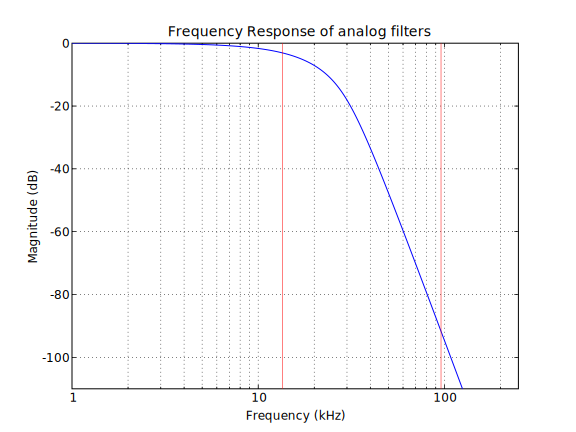
\includegraphics[scale=1.0]{soma-1.analog.freqres.svg}
  \label{analog.freqres}
  \caption{Anti-aliasing filter total frequency response.}
\end{figure}

\begin{figure}[h!]
  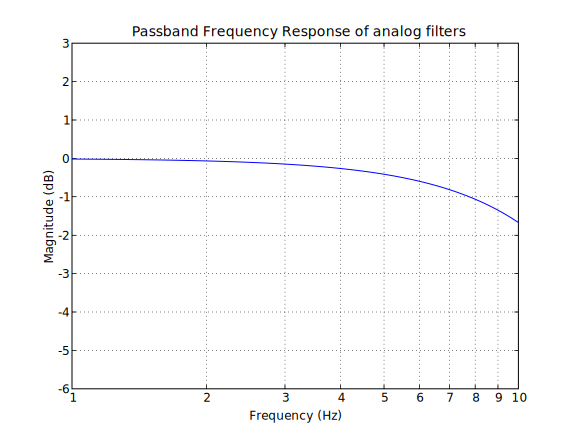
\includegraphics[scale=1]{soma-1.analog.pass.svg}
  \label{analog.pass}
  \caption{Antialiasing filter passband frequency response}
  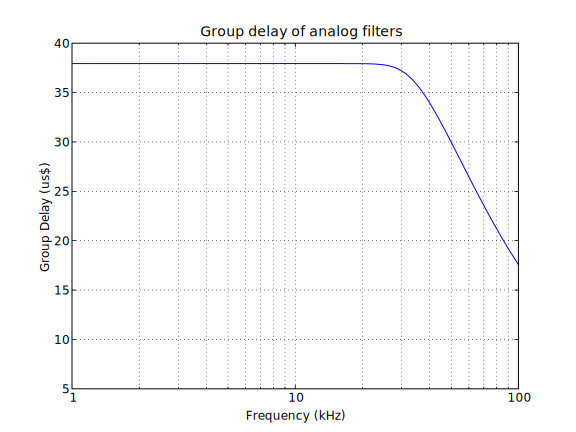
\includegraphics[scale=1.0]{soma-1.analog.grd.svg}
  \label{analog.grd}
  \caption{Anti-aliasing filter group delay.}
\end{figure}

\subsection{ADC}
A 16-bit ADC running at $f_s=192 \textrm{kHz}$ samples the incoming antialiased signal. 

\subsection{Filtering}
We filter the sampled data using an N-Tap FIR filter using fixed-point
convolution. We use an extended-precision multiplier, 22-bit filter
coefficients, and an extended-width accumulator to reduce the negative
artifacts present in fixed-point aritmetic.

The Parks-McClellan optimum equiripple FIR filter is used for a cutoff
at 10 kHz; the resulting frequency response (and coefficient-quantized
frequency response) are seen in figure \ref{FIR}. A 143-tap filter
gives the required stopband attenuation while keeping FIR-induced
passband ripple to under $0.5 dB$, while fitting in our allocated FPGA
resources.

\begin{figure}[h!]
  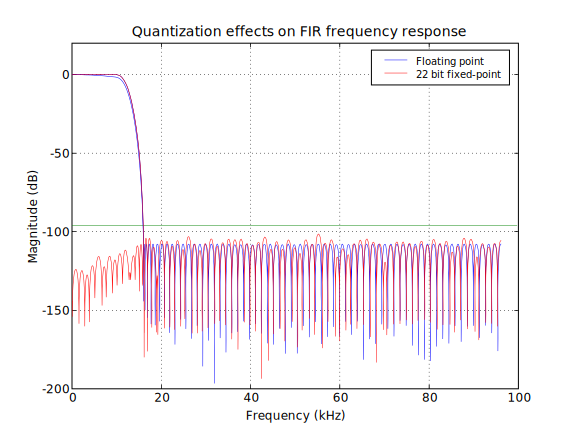
\includegraphics[scale=1.0]{soma-1.digital.quant.svg}
  \label{FIR}
  \caption{Frequency response of FIR filter.}
\end{figure}

\subsection{Downsampling}
We filter and then downsample; the filtering step is actually only
performed once for every $M=6$ input samples, as the other $M-1$
samples would be removed in the decimation step and thus be wasted.

\subsection{Total response, designed and measured}
The resulting frequency response of the combined analog and digital
filters are shown in figures blah, including zoomed-in passband and
stopband performace. The frequency response following decimation is
also shown, with the sum of the (imperfectly filtered) antialiased
components highlighted.

\begin{figure}[h!]
  \includegraphics[scale=1.0]{soma-1.digital.aggregate.svg}
  \label{digital.aggregate}
  \caption{Aggregate pre-decimation signal chain filtering.}
  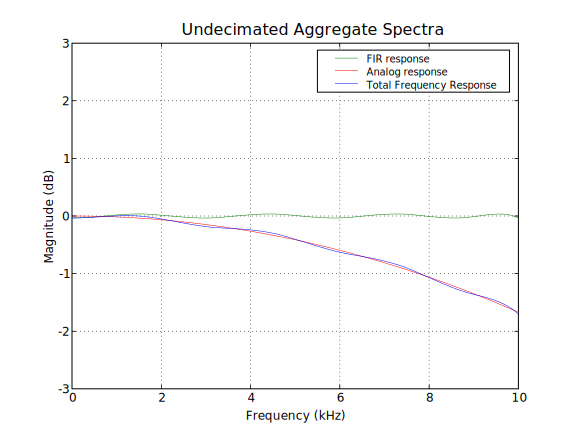
\includegraphics[scale=1.0]{soma-1.digital.pass.svg}
  \label{digital.pass}
  \caption{Aggregate pre-decimation signal chain passband.}
\end{figure}


\begin{figure}[h!]
  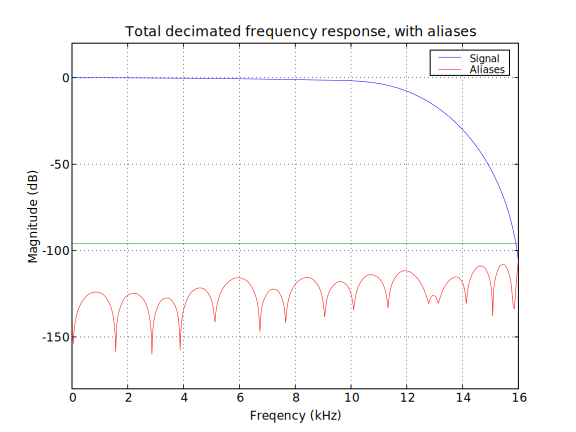
\includegraphics[scale=1.0]{soma-1.digital.withaliases.svg}
  \label{digital.withaliases}
  \caption{Aggregate post-decimation filtering.}
\end{figure}


Frequency Response measurements THD+N Measurements

